\documentclass{article}
\usepackage[utf8]{inputenc}
\usepackage{amsmath,amsthm,amssymb}
\usepackage[dutch]{babel}
\usepackage{float}
\usepackage{longtable}
\usepackage{graphicx}
\usepackage{xcolor}
\usepackage[labelfont=bf,justification=centering]{caption}
\usepackage[framed,numbered,autolinebreaks,useliterate]{mcode}

\begin{document}
\begin{titlepage}
	
	\newcommand{\HRule}{\rule{\linewidth}{0.5mm}}
	
	\center
	
	\textsc{\LARGE Katholieke Universiteit Leuven}\\[1.5cm]
	\textsc{\Large Bachelor informatica}\\[0.5cm]
	\textsc{\large Numerieke Wiskunde}\\[0.5cm]
	
	\HRule \\[0.4cm]
	{ \huge \bfseries Practicum QR-Algoritme }\\[0.4cm]
	\HRule \\[1.5cm]
	\begin{minipage}
		{0.4
		\textwidth} 
		\begin{flushleft}
			\large \emph{Door:}\\
			Robin \textsc{Haveneers} \\
			\emph{r0450702}\\
			Mathias \textsc{Van Herreweghe} \\
			\emph{r0456156}
		\end{flushleft}
	\end{minipage}
	~ 
	\begin{minipage}
		{0.4
		\textwidth} 
		\begin{flushright}
			\large \emph{In opdracht van:} \\
			Professor \\
			Marc \textsc{Van Barel} 
		\end{flushright}
	\end{minipage}
	\\[4cm]
	
	{\large Academiejaar 2015 - 2016}\\
	\begin{figure}
		[b] \centering 
		\includegraphics[scale = 0.2]{kul.png} 
	\end{figure}
\end{titlepage}

\tableofcontents
\newpage
\section*{Inleiding}
Het doel van dit practicum is het implementeren van het $QR$-algoritme voor het berekenen van de eigenwaarden van een matrix. We zullen stapsgewijs kennis maken met de bouwstenen die hiervoor nodig zijn. Dit bevat zowel theoretische bewijzen als praktische code in Matlab. We beschrijven uitvoerig de werking van onze bevindingen, alsook beargumenteren we verschillende eigenschappen van de $QR$-algoritmen.

\newpage

%%%%%%%%%%%%%%%%%%%%%%%%%%%%
%%%% DE QR-DECOMPOSITIE %%%%
%%%%%%%%%%%%%%%%%%%%%%%%%%%%

\section{De $QR$-Decompositie}

\subsubsection*{Vraag 1}
% Beschrijving van het algoritme hoe je tot een bovendriehoeksmatrix R en matrix Q komt.

Het algoritme begint met $\text{r}_{1,1}$ gelijk te stellen aan de lengte van de eerste kolom van $A$.
Daarna stelt het algoritme de eerste kolom van $Q$ gelijk aan de eerste kolom van $A$ gedeeld door de norm van de eerste kolom van A.\\

Vervolgens wordt in de binnenste for-lus bij elke iteratie elementen met de waarde $(\mathbf{q}_i)^T * \mathbf{a}_{j+1}$ boven de diagonaal in de kolom $j+1$ van $R$ geplaatst. De lus beperkt zich tot de elementen boven de diagonaal door de index $i$,die voor de rij gebruikt wordt, niet hoger te laten worden dan de index $j$ van de buitenste lus, die als kolom-index dient.\\

Na de uitvoering van de binnenste for-lus wordt in de omvattende for-lus bij elke iteratie een diagonaal-element van $R$ ingevuld op plaats $\text{r}_{j+1,j+1}$. De waarde van dit diagonaal-element in $R$ is 
\begin{center}
$\mathbf{a}_{j+1} - (\sum\limits_{i=1}^j \text{r}_{i,j+1} * \mathbf{q}_i)$.
\end{center}


In een wiskundigere notatie krijgen we door het Gram-Schmidt process de vectoren  $ {\mathbf u}_1, {\mathbf u}_2, \ldots, {\mathbf u}_n$ die de vectoren in $Q$ voorstellen, alsook
\begin{center}
$\displaystyle R = \begin{bmatrix}{\alpha}_{11} & {\alpha}_{12} & \cdots & {\alpha}_{1n}\\
0 & {\alpha}_{22} & \cdots & {\alpha}_{2n} \\
\vdots & \vdots & \ddots & \vdots \\
0 & 0 & \cdots & {\alpha}_{nn} \end{bmatrix}.$
\end{center}
Zo krijgen we dus
\begin{center}
	$ QR = [{\mathbf u}_1, {\mathbf u}_2, \ldots, {\mathbf u}_n] \begin{bmatrix}{\alpha}_{11} & {\alpha}_{12} & \cdots & {\alpha}_{1n}\\
0 & {\alpha}_{22} & \cdots & {\alpha}_{2n} \\
\vdots & \vdots & \ddots & \vdots \\
0 & 0 & \cdots & {\alpha}_{nn} \end{bmatrix}$\\
\vspace{5mm}
$ = \biggl[ {\alpha}_{11} {\mathbf u}_1 , {\alpha}_{12} {\mathbf u}_1 + {\alpha}_{22} {\mathbf u}_2 , \ldots , \sum\limits_{i=1}^n \alpha_{in}{\mathbf u}_i \biggr]$\\
\vspace{3mm}
$ = [{\mathbf a}_1, {\mathbf a}_2, \ldots, {\mathbf a}_n] = A$. 

\begin{itemize}
\item We kunnen nu aantonen dat Q \textbf{orthogonaal} is:\\
Neem $q_1 = \frac{a_1}{\parallel a_1 \parallel}$ en neem ook zoals in het algoritme $z^{(2)} = a_2 - q^T_1a_2q_1.$ De kolommen van $Q$ moeten nu een orthonormaal stelsel vormen omdat $Q$ orthogonaal is. De dus de kolommen staan loodrecht op elkaar en hebben lengte (norm) 1. Dit geldt voor kolom 1 en 2, volgens het volgende bewijs via inproduct.
\begin{align*}
< z^(2), q_1 > & = z^(2)^Tq_1\\
&= (a_2 - q^T_1a_2q_1)q_1\\
& \vdots\\
&= 0
\end{align*}
\item We kunnen ook vrij eenvoudig aantonen dat R \textbf{een bovendriehoeksmatrix} is. Er geldt namelijk dat $ i>j$ en dus $R_{ij} = 0$.
\end{itemize}

%QR=A
\end{center}

\subsubsection*{Vraag 2}
% beschrijving van de algoritmes, hoe het komt dat deze 2 algoritmes theoretisch (niet numeriek!) equivalent zijn. (dus niet volgens 2.3 p.48 in het handboek)

We analyseren de gegeven (pseudo-)code. Laten we de som uitschrijven die voorkomt in de eerste versie van het Gram-Schmidt algoritme.
\begin{align*}
    z &= z - \sum_{i=1}^j r_{i,j+1}q_i \\
    &= z - (r_{1,j+1}q_1 + r_{2,j+1}q_2 + \dots + r_{j,j+1}q_j)
\end{align*}

Schrijven we nu de lijn $z=z-r_{i,j+1}q_i$ uit de binnenste for-lus van het Modified Gram-Schmidt algoritme eens uit dan krijgen we het volgende.
\begin{itemize}
\item Na \'e\'en iteratie door de binnenste for lus is de variabele $z = z - r_{1,j+1}q_1$.
\item Na een tweede iteratie is $z = z- r_{1,j+1}q_1 - r_{2,j+1}q_2$\\
\vdots
\vspace{-1mm}
\item Na $j$ iteraties is $z = z - r_{1,j+1}q_1 - r_{2,j+1}q_2 + \dots - r_{j,j+1}q_j$
\end{itemize}
In onze algoritmes heeft $z$ uiteraard ook een waarde, maar deze is niet van belang om in te zien dat de for-lus en de som tot exact hetzelfde resultaat komen.

\subsubsection*{Vraag 3}
De implementatie van het klassieke Gram-Schmidt algoritme vind je hieronder.
\vspace{-5mm}
\begin{lstlisting}
function [Q,R] = gramschmidt1(A)
R(1,1) = norm(A(:,1));
Q(:,1) = A(:,1)/(R(1,1));
[~,n] = size(A);
for k = 1:(n-1)
    z=A(:,k+1);
    for l = 1:k
        R(l,k+1) = (Q(:,l)')*z;
    end
    z = z-specialsum(Q,R,k);
    R(k+1, k+1) = norm(z);
    Q(:,k+1) = z./(R(k+1,k+1));
end
Q
R
end
\end{lstlisting}

De hulpfunctie \texttt{specialsum}, vind je hier.
\vspace{-5mm}
\begin{lstlisting}
function a = specialsum(Q,R,m)
a = 0;
for p = 1:m
    a = a + R(p,m+1)*Q(:,p);
end
end
\end{lstlisting}

De code voor het aangepaste of 'modified' Gram-Schmidt algoritme vind je hieronder.
\vspace{-5mm}
\begin{lstlisting}
function [Q,R] = gramschmidt2(A)
R(1,1) = norm(A(:,1));
Q(:,1) = A(:,1)/(R(1,1));
[~,n] = size(A);
for k = 1:(n-1)
    z=A(:,k+1);
    for l = 1:k
        R(l,k+1) = (Q(:,l))'*z;
        z = z - R(l,k+1)*Q(:,l);
    end
    R(k+1, k+1) = norm(z);
    Q(:,k+1) = z./(R(k+1,k+1));
end
Q
R
end
\end{lstlisting}

Om duidelijk te maken welk van de twee algoritmes het meest nauwkeurige resultaat geeft, hebben we de relatieve fout berekend. We hebben voor elk van de twee implementaties (Gram Schmidt 1 en modified Gram Schmidt) telkens de relatieve fout berekend ten opzichte van de ingebouwde \texttt{qr}-functie in Matlab zelf. Hiervoor hebben we telkens de matrices omgevormd naar vectoren door de rijen achter elkaar te plaatsen om zo eenvoudig de relatieve fout te kunnen berekenen en te plotten. Het resultaat daarvan zie je in onderstaande figuren.
\begin{figure}[H]
\centering
    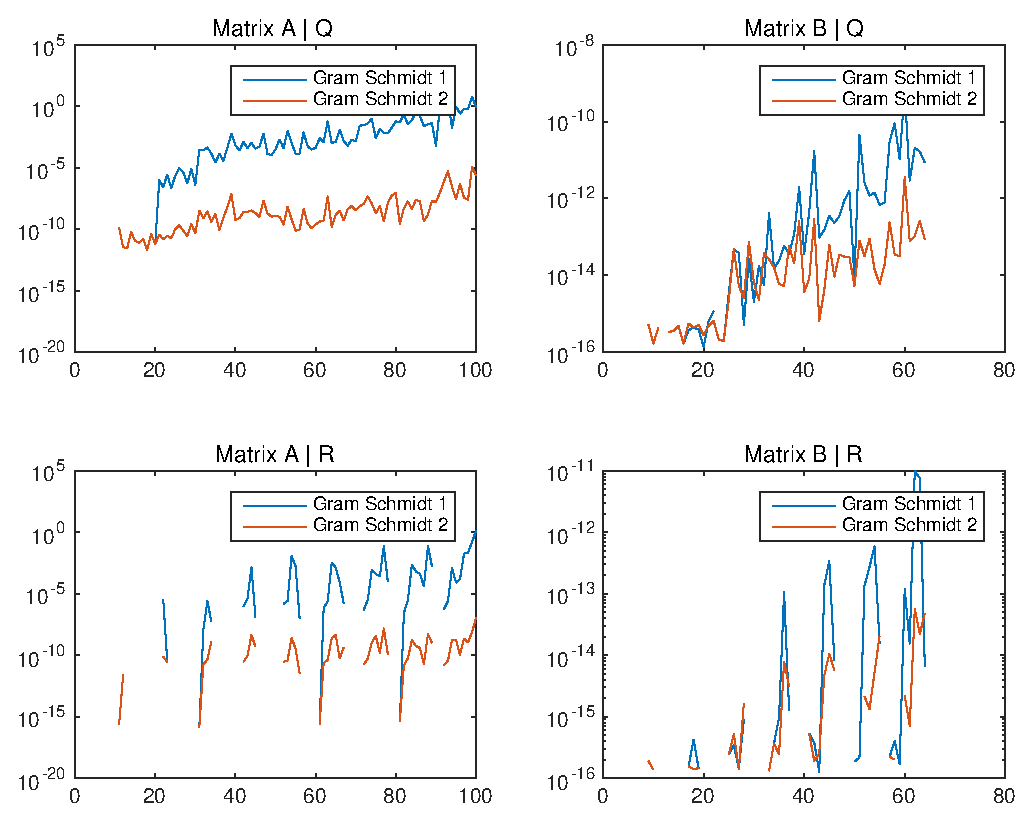
\includegraphics[width=\linewidth]{GramSchmidtRelError} 
    \caption{Relatieve fout van Gram Schmidt\\ten opzichte van Matlab's QR functie}
\end{figure}

De verklaring voor het verschil in de nauwkeurigheid ligt in het feit dat in het klassieke Gram-Schmidt algoritme we de lengtes berekenen van de orthogonale projecties van $z=a_{j+1}$ op $q_1,q_2,...q_{n-1}$ om nadien de projecties (en de bijhorende afrondingsfouten) af te trekken van z. Stel $Q_{n-1} = \{q_1,q_2,\dots,q_{n-1}\}$, dan is de orthogonale projectie op de kolomruimte van $Q_{n-1}$ gelijk aan $P=Q_{n-1}(Q^t_{n-1}Q_{n-1})^{-1}Q^t_{n-1}$. Als $Q_{n-1}$ orthonormale kolommen heeft, dan is $P=Q_{n-1}Q^t_{n-1}:$ 
$$w = (I-Q_{n-1}Q^t_{n-1})a_{j+1}.$$
Maar omwille van afrondingsfouten, heeft $Q_{n-1}$ geen `echte' orthogonale kolommen. In het Modified Gram-Schmidt algoritme berekenen we de lengte van de projectie $z=a_{j+1}$ op $q_1$ en trekken we die projectie (en de afrondingsfouten) af van $z$. Vervolgens berekenen we de lengte van de projectie van de reeds \textit{berekende} $z$ op $q_2$ en trekken die projectie (en de afrondingsfouten) af van $z$, en zo verder, maar altijd na orthogonalisatie ten op zichte van de reeds \textbf{berekende versie} van $z$. Evalueren we nu van rechts naar links:
$$z = (I-q_{n-1}q_{n-1}^t) \dots (I-q_2q_2^t)(I-q_1q_1^t)a_n.$$
Als de berekende $Q^t_{n-1}Q_{n-1} = I + E$, dan is deze $z$ zo goed als dezelfde dan als ze wordt berekend met $$z=(I-Q_{n-1}(Q^t_{n-1}Q_{n-1})^{-1}Q^t_{n-1})a_k$$ waar we $(Q^t_{n-1}Q_{n-1})^{-1}$ vervangen door $I-E$, en deze is ook meer `orthogonaal' ten opzichte van $Q_{n-1}$ dan de $z$ bekomen in het klassieke algoritme.



%%%%%%%%%%%%%%%%%%%%%%%%%%%%%%%%
%%%% HET BASIS QR ALGORITME %%%%
%%%%%%%%%%%%%%%%%%%%%%%%%%%%%%%%

\section{Het basis $QR$-algoritme}
\subsubsection*{Vraag 1}
\textbf{Toon aan dat de matrices $A_0, A_1, \dots$ dezelfde eigenwaarden hebben.}\\
\\
\noindent\textbf{Bewijs :}
We weten dat twee matrices gelijkvormig zijn als en slechts als er een inverteerbare matrix $P$ bestaat zodat $A=P^{-1}BP$ en we weten dat gelijksoortige matrices dezelfde eigenwaarde hebben. We tonen dit aan.\\
Stel $A=P^{-1}BP$ dan kan men de eigenwaarden halen uit $det(A- \lambda I) = 0 $. Er volgt nu:
\begin{align*}
    0 &= \det(A- \lambda I) \\
    &= \det(P^{-1}(B- \lambda I)P)\\
    &= \det(P^{-1})\det(P)\det(B - \lambda I) \tag{En: $\det(P^{-1})\det(P) = 1$} \\
    &= \det(B - \lambda I)
\end{align*}
Matrices met dezelfde karakteristieke veelterm hebben dezelfde eigenwaarden. We bewijzen nu dat $A_1, A_2,\dots$ gelijksoortige matrices zijn. Aangezien:
\begin{align*}
    A_{k+1} &= R_k Q_k \\
    &= (Q^T_k Q_k)R_kQ_k \tag{$Q$ is een orthogonale matrix is, er geldt $Q^T Q = I$}\\
    &= Q^T_k (Q_kR_k)Q_k\\
    &= Q^T_k (A_k)Q_k\\
    &= Q^{-1}_k (A_k)Q_k \tag{$Q$ is een orthogonale matrix is, er geldt $Q^T=Q^{-1}$}
\end{align*}
Er geldt nu dat $A_{k+1} = Q^{-1}_k (A_k)Q_k$ wat betekent dat $A_k en A_{k+1}$ gelijksoortige matrices zijn. We hebben hierboven aangetoond dat gelijksoortige matrices dezelfde karakteristieke veelterm en dus dezelfde eigenwaarden hebben.\qed

\subsection*{Vraag 2}
De code hieronder is de code voor \texttt{QRstep.m}.
\vspace{-5mm}
\begin{lstlisting}
function [A] = QRstep(I)
[Qi,Ri] = qr(I); 
A = Ri*Qi;
A = max(A, eps);
figure;
imagesc(A);
hold on;
end
\end{lstlisting}

\newpage

\subsection*{Vraag 3}
\begin{itemize}
    \item In de bovenstaande vier figuren (figuur 2) zie je de visualisatie van  $A_k$ met \texttt{imagesc} voor een random symmetrische matrix A met eigenwaarden $\lambda_i = \{1,2,4,8,16,256,512,2048\}$.
    
\begin{figure}   
\begin{center}
    \includegraphics[width=.4\textwidth]{im1}
    \includegraphics[width=.4\textwidth]{im2}
    \includegraphics[width=.4\textwidth]{im3}
    \includegraphics[width=.4\textwidth]{im4}
\end{center}
\caption{Visualisatie van (linksboven naar rechtsonder): $A_1$,$A_2$,$A_3$,$A_4$.}
\end{figure}

\item In de volgende 11 figuren zie je het lineaire convergentiegedrag. Dit is bekomen door de diagonaalmatrix op te stellen die dient bekomen te worden en zo per qr-stap de absolute fout te berekenen met de matrix in die stap. 

\begin{figure}
\vspace{-2.1cm}
\begin{center}
\caption{Visualisatie van lineaire convergentie. Linksboven naar rechtsonder: voor de qr-stappen, stap 1 t.e.m. 9 en de laatste afbeelding is het resultaat.}
    \includegraphics[width=.4\textwidth]{before}
    \includegraphics[width=.4\textwidth]{1}
    \includegraphics[width=.4\textwidth]{2}
    \includegraphics[width=.4\textwidth]{3}
    \includegraphics[width=.4\textwidth]{4}
    \includegraphics[width=.4\textwidth]{5}
    \includegraphics[width=.4\textwidth]{6}
    \includegraphics[width=.4\textwidth]{7}
    \includegraphics[width=.4\textwidth]{8}
    \includegraphics[width=.4\textwidth]{9}
    \includegraphics[width=.4\textwidth]{after}
\end{center}

\end{figure}
    
\end{itemize}

Als we onze \texttt{QRstep} uitvoeren op de matrix B dan krijgen we op de diagonaal de correcte eigenwaarden, behalve op twee plaatsen. De 5\textsuperscript{e} en 6\textsuperscript{e} eigenwaarde zijn 0, na het uitvoeren van de \texttt{QRstep}. Dit is te wijten aan het feit dat deze eigenwaarden complex zijn in de originele matrix, zoals te zien met \texttt{eig(B)}, hieronder.

\begin{table}[H]
\fontfamily{pcr}\selectfont
\begin{tabular}{rcr}
   1.0e+03 $*$&&\\
   2.0480 &+ &0.0000i\\
   0.5120 &+ &0.0000i\\
   0.2560 &+ &0.0000i\\
   0.0160 &+ &0.0000i\\
   {\color{red} -0.0000} &{\color{red}+} &{\color{red}0.0080i}\\
   {\color{red}-0.0000} &{\color{red}-}&{\color{red}0.0080i}\\
  -0.0000 &- &0.0080i\\
   0.0020 &+ &0.0000i\\
   0.0010 &+ &0.0000i
   \end{tabular}
   \end{table}

\subsection*{Vraag 4}
In de functie \texttt{QRstep} gebeurt de standaard \texttt{qr}-functie van Matlab gevolgd door een matrix vermenigvuldiging. De \texttt{QRstep} van Matlab is $O(n^3)$, en hetzelfde geldt voor de matrix vermenigvuldiging van Matlab. We kunnen dus besluiten dat de totale complexitieit $O(n^3)$ is.

\section{ Het $QR$-algoritme: twee fasen}

\subsection{Fase 1: Householder transformaties}
\subsubsection*{Vraag 1}
\begin{align*}
    K&=Q*R\\
    Q^TK&=Q^TQR \\
    Q^TK&=R  \tag{$Q^TQ=I$ aangezien $Q$ orthogonaal is.}\\
    R &= 
    \begin{pmatrix}
        | & | & | &  & |\\
        Q^{T}x & Q^{T}Ax & Q^TA^2x & \cdots & Q^TA^{n-1}x \\
        | & | & | &  & |\\
    \end{pmatrix}
\end{align*}
Vervolgens kan men $Q^TQ=I$ vermenigvuldigen met elk element. Dit geeft
 \[
 R =
 \begin{pmatrix}
 \centering
        | & | & | &  & |\\
        Q^Tx& (Q^TAQ)Q^Tx& (Q^TAQ)^2Q^Tx & \cdots &(Q^TAQ)^{n-1}Q^Tx) \\
        | & | & | &  & |\\
\end{pmatrix}
\]

Dit in combinatie met $Q^TK=R$ geeft
\[
Q^TK =
\begin{pmatrix}
\centering
        | & | & | &  & |\\
        Q^Tx & (Q^TAQ)Q^Tx & (Q^TAQ)^2Q^Tx  & \cdots & (Q^TAQ)^{n-1}Q^Tx  \\
        | & | & | &  & |\\
\end{pmatrix}
\]

Ook merken we op dat aangezien $Q^TK=R$ en R een bovendriehoeksmatrix is volgens het gegeven, is $Q^TK$ dat ook.

In de laatste vermeldde matrix is elke kolom gelijk aan $(Q^TAQ)$ vermenigvuldigd met de vorige kolom, met triviale uitzondering van de eerste kolom.

Aangezien $Q^TAQ=H$ voldoet H dus aan bovenvermelde eigenschap betreffende de structuur van de kolommen. Bijgevolg is $H$ dus een Hessenberg-matrix.



\subsubsection*{Vraag 2}


\textbf{Bewijs: Householder transformatie is symmetrisch en orthogonaal.}
\textbf{Symmetrisch}\\
We willen aantonen dat $P^T=P$.
\begin{align*}
    P^T &= (I - 2uu^T)^T \\
    &= I^T - (2uu^T)^T\\
    &= I - 2(u^T)^Tu^T\\
    &= I - 2uu^T\\
    &= P
\end{align*}
\textbf{Orthogonaal}\\
We willen aantonen dat $PP^T=I$.
\begin{align*}
    PP^T &= (I - 2uu^T)(I - 2uu^T)^T \\
    &= (I - 2uu^T)(I - 2uu^T) \tag{$P=P^T$ volgens symmetrie}\\
    &= I - 4uu^T + 4uu^Tuu^T\\
    &= I - 4uu^T + 4u(u^Tu)u^T\\
    &= I - 4uu^T + 4uu^T \tag{$\parallel{u}\parallel = u^Tu = 1$}\\
    &= I
\end{align*}
\qed
\subsubsection*{Vraag 3}
We zullen dit aantonen door naar het spiegelbeeld $Px$ van $x$ rond het vlak loodrecht op $u$ toe te werken.

We nemen de vector $u$ vector waarop we loodrecht een hypervlak nemen waarrond de reflectie gebeurt. We schrijven de vector $x$ die we spiegelen rond $\textbf{u}^{\bot}$ als de som $x = \lambda{}u + v$ met $v \in u^{\bot}$. Nu willen we $\lambda \in \mathbb{R}$ kiezen zodat $u \cdot x = \lambda u\cdot u + u\cdot v = \lambda$. Zo volgt $x = (u \cdot x)u + v$.
Als we $x$ willen reflecteren rond $u^{\bot}$, trekken we twee keer diens $u$-component er van af:
\begin{align*}
Px= x-2(u \cdot x)u = x- 2u(u^Tx) = (I-2uu^T)x
\end{align*}
Hierbij is aangetoond dat de (orthogonale) reflectie rond een hypervlak $u^{\bot}$ van de vorm $P = I-2uu^T$ is.

\begin{figure}[H]
\begin{center}
   \includegraphics[width=.4\textwidth]{reflector_schets}
   \caption{Illustratie van een Householder reflector, met spiegelbeeld $Px$ van $x$.}
\end{center}
\end{figure}

\subsubsection*{Vraag 4}

Vanuit het gegeven weten we dat 
\begin{align*}
    u=\frac{x+\alpha e_1}{\parallel x+\alpha e_1\parallel} = \frac{z}{\parallel z \parallel} \text{ met } \alpha = \rho \parallel x \parallel.
\end{align*}
Hiermee berekenen we dat
\begin{align*}
    z^Tz = (x-\alpha e_1)^T(x-\alpha e_1) = 2(\parallel x \parallel^2+\rho \parallel x \parallel x_1).
\end{align*} 
Daarnaast is 
\begin{align*}
    z^Tx=\parallel x \parallel^2+\rho \parallel x \parallel x_1.
\end{align*} 
Hieruit volgt
\begin{align*}
    uu^Tx=\frac{z}{\parallel z \parallel} \frac{z^T}{\parallel z \parallel}x=\frac{z^Tx}{Z^Tz}z=\frac{\parallel x \parallel^2+\rho \parallel x \parallel x_1}{2(\parallel x \parallel^2+\rho \parallel x \parallel x_1)}z=\frac{1}{2}z
\end{align*}
Waaruit we halen dat
\begin{align*}
    Px=(I-2uu^T)x=x-2uu^Tx=x-z\\
    =x-(x+\alpha e_1)=-\alpha e_1 = -\rho \parallel x \parallel e_1.
\end{align*}

\subsubsection*{Vraag 5}
In het eerste deel van de vraag beschouwen een matrix die we $P_1$ noemen en we geven deze gemakkelijkheidshalve de vorm
\begin{align*}
    P_1=
    \begin{bmatrix}
    1 & 0 & 0 & 0 & 0\\
    0 & \times & \times & \times & \times\\
    0 & \times & \times & \times & \times\\
    0 & \times & \times & \times & \times\\
    0 & \times & \times & \times & \times\\
    \end{bmatrix}
    =
    \begin{bmatrix}
    1 & 0^T\\
    0 & I-2u_1u_1^T\\
    \end{bmatrix}
\end{align*}
Een gevolg van het gegeven is dat
\begin{align*}
    (I-2u_1u_1^T)\begin{bmatrix}a_{21}\\\vdots\\a_{n1}\end{bmatrix}=\alpha e_1.
\end{align*}
Hieruit volgt rechtstreeks dat $P_1$ vermenigvuldigd met $A$ de nullen in de eerste kolom plaatst, buiten in de eerste 2 rijen. Zo krijgen we
\begin{align*}
    P_1A=
    \begin{bmatrix}
    \times & \times & \times & \times & \times\\
    \times & \times & \times & \times & \times\\
    0 & \times & \times & \times & \times\\
    0 & \times & \times & \times & \times\\
    0 & \times & \times & \times & \times\\
    \end{bmatrix}.
\end{align*}
Door de symmetrie van Householder reflectoren weten we dat $P_1^T=P_1$. Hieruit volgt dat $P_1AP_1^T=P_1AP_1$. Door de niet-nul structuur van $P_1$ blijft de niet-nul structuur van $P_1AP_1$ ongewijzigd. Zo krijgen we de matrix
\begin{align*}
    P_1AP_1=
    \begin{bmatrix}
    \times & \times & \times & \times & \times\\
    \times & \times & \times & \times & \times\\
    0 & \times & \times & \times & \times\\
    0 & \times & \times & \times & \times\\
    0 & \times & \times & \times & \times\\
    \end{bmatrix}.
\end{align*}
die orthogonaal gelijkvormig is aan A en de eerste kolom in alle rijen nullen bevat behalve in de eerste twee.

Het proces kunnen we vervolgen door te stellen dat 
\begin{align*}
    P_2=\begin{bmatrix}
    1 & 0 & 0^T\\
    0 & 1 & 0^T\\
    0 & 0 & I-2u_2 u_2^T\\
    \end{bmatrix}.
\end{align*}
waarbij $u_2$ gemaakt wordt uit de $n-2$ laatste elementen uit de tweede kolom van $P_1AP_1^T$. Dan krijgen we 
\begin{align*}
    P_2P_1AP_1P_2=
    \begin{bmatrix}
    \times & \times & \times & \times & \times\\
    \times & \times & \times & \times & \times\\
    0 & \times & \times & \times & \times\\
    0 & 0 & \times & \times & \times\\
    0 & 0 & \times & \times & \times\\
    \end{bmatrix}
\end{align*}
Als we analoog te werk gaan krijgen we uiteindelijk na $n-2$ stappen
\begin{align*}
    P_{n-2}P_{n-3}\dots P_2P_1AP_1P_2\dots P_{n-2}=H,
\end{align*}
waarbij $H$ de gewenste Hessenberg matrix is, en dus orthogonaal equivalent is met A.

\subsubsection*{Vraag 6}%
Als we onze \texttt{Householder.m} testen op random Hermitische matrices, met de volgend code:
\vspace{-5mm}
\begin{lstlisting}
Hermitisch = cell(6,1);

for l=4:10
    A = complex(randn(4,4));
    Hermitisch{l-3} = (A + A')/2;
end

for l=1:6
    test = Hermitisch{l}
    Householder(Hermitisch{l})
end
\end{lstlisting}
Dan verkrijgen we steeds Hessenberg matrices die zowel boven als onder de respectievelijke bovenste en onderste subdiagonaal nullen hebben staan. Er ontstaat een tri-diagonale matrix.

Een voorbeeld hiervan vind je hieronder.
\vspace{-5mm}
\begin{lstlisting}
>> Householder(a)

ans =

   1.3363  1.0246  0.0000  -0.0000
   1.0246 -0.8848  1.0201  -0.0000
   0       1.0201  0.6541   1.4192
   0      -0.0000  1.4192  -1.2469
  
\end{lstlisting}

\subsection{Fase 2: $QR$-stap op Hessenberg matrix}
\label{subsec:Fase2}
\subsubsection*{Vraag 1}
De Givens rotaties zijn van de vorm:
\begin{align*}
G_1=\begin{bmatrix}
        \hat{G_1} & 0\\
        0 & I_{n-2}\\
    \end{bmatrix},
G_2=\begin{bmatrix}
        1 & 0 & 0\\
        0 & \hat{G_2} & 0\\
        0 & 0 & I_{n-3}\\
    \end{bmatrix}, \cdots
\end{align*}
met $\hat{G_i}$ zodanig dat als deze vermenigvuldigd wordt met $G_{i-1} \cdots G_{1}A$, de uitkomst leidt tot een matrix die tot op de $(i+1)$-de rij voldoet aan een bovendriehoeksmatrix.

Door dit te doen tot op de $n$-de rij (dus na $(n-1)$ rotaties) verkrijgen we de QR-decompositie van A, met

\[\underbrace{G_{n-1} \cdots G_{2}G_{1}}_{Q^T}A=
\begin{bmatrix}
    \times & \times & \times & \times & \times\\
    0 & \times & \times & \times & \times\\
    0 & 0 & \times & \times & \times\\
    0 & 0 & 0 & \times & \times\\
    0 & 0 & 0 & 0 & \times\\
 \end{bmatrix}\]
en
\begin{align*}
    Q=G_1^{-1}G_2^{-1}\cdots G_{n-1}^{-1} \text{ en } R=Q*A.
\end{align*}
Daarna berekenen we het product $R*Q$, namelijk
\begin{align*}
    H=R*Q=RG_1^{-1}G_2^{-1} \cdots G_{n-1}^{-1}=RG_1^{T}G_2^{T} \cdots G_{n-1}^{T}\\
\end{align*}
Hierin is dus duidelijk te zien dat er $n-1$ Givens rotaties nodig zijn. 
\subsubsection*{Vraag 2}
De matrix die bekomen wordt na het uitvoeren van \texttt{QRstep.m} op een Hessenberg matrix, geeft opnieuw een Hessenberg matrix.\\

\noindent\textbf{Stelling:} Laat $A_k$ een boven-Hessenberg matrix zijn en laat $A_k=Q_{k}R_{k}$ de QR-factorizatie zijn van $A$. Dan is $A_{k+1}=R_{k}Q_{k}$ ook een boven-Hessenberg matrix.\\
\noindent\textbf{Bewijs:} Veronderstel dat Givens rotaties zijn gebruikt voor het factorizeren van $A_k$ in $Q_{k}R_{k}$. Dan is
\[Q_k=G_1^{-1}G_2^{-1}\cdots G_{n-1}^{-1}\]
ook een boven-Hessenberg.

Aangezien $R_k$ een bovendriehoeksmatrix is en $Q_k$ boven-Hessenberg, is $A_{k+1}=R_{k}Q_{k}$ ook boven-Hessenberg.\qed
\subsubsection*{Vraag 3}

De code hieronder is de code voor \texttt{QRstepHessenberg.m}.
\vspace{-5mm}
\begin{lstlisting}
function [Hk] = QRstepHessenberg(H)
[M,N] = size(H);
Qstar = H;
Q=eye(M,N);
for l = 1:N-1
    subMatrix = [H(l,l), H(l+1,l)]';
    [Gr,~] = planerot(subMatrix);
    G = eye(M,N);
    G(l:l+1,l:l+1) = Gr(1:2,1:2); 
    Qstar =  G * Qstar;
    Q = Q * G^-1;
end
Hk = Qstar*Q;
end
\end{lstlisting}

\subsubsection*{Vraag 4}
Het toepassen van een Givens rotatie kan gedaan worden in $\mathcal{O}(n)$. Zoals reeds aangetoond in vraag 1 van deze subsectie (\ref{subsec:Fase2})  dienen we twee keer deze Givens rotaties toe te passen, op deze manier krijgen we dus $\mathcal{O}(n*n)=\mathcal{O}(n^2)$.


\subsubsection*{Vraag 5}
De code hieronder is de code voor \texttt{generalQRstep.m}.
\vspace{-5mm}
\begin{lstlisting}
function [Hk] = GeneralQRstep(H,k)
House = Householder(H);
for l = 1:k
    Hk = QRstepHessenberg(House);
end
\end{lstlisting}


\newpage
\subsubsection*{Vraag 6}
Het experiment is als volgt opgezet. 
\begin{itemize}
    \item Genereer de matrixen die we gaan evalueren\\
    \vspace{-5mm}
    \begin{lstlisting}
n  = round(logspace(1,3,10));
matrices = cell(9,1);

for l = 1:9
    matrices{l} = rand(n(l));
end
    \end{lstlisting}
    \item Time de \texttt{generalQRstep.m}-methode\\
    \vspace{-5mm}
    \begin{lstlisting}
tijd_general = zeros(9,1);
for l = 1:9
    tic
    GeneralQRstep(matrices{l},100);
    tijd_general(l) = toc;
end
    \end{lstlisting}
    \item Time tenslotte de gewone \texttt{QRstep}-methode.\\
    \vspace{-5mm}
    \begin{lstlisting}
tijd_qr = zeros(9,1);
for l = 1:9
    tic
    for k = 1:100
        matrices{l} = QRstep(matrices{l});
    end
    tijd_qr(l) = toc;
end
    \end{lstlisting}
\end{itemize}

Het resultaat zie je in onderstaande grafiek.

\begin{figure}[H]
\includegraphics[width=\linewidth]{laatsteplot}
\caption{Vergelijking \texttt{QRstep} - \texttt{generalQRstep}}
\end{figure}

\section{Tijdsbesteding}

\begin{longtable}{l|c|c|}
  & Mathias & Robin \\
 \hline
\endfirsthead
\endhead
\multicolumn{2}{r}{{Continued\ldots}} \
\endfoot
\hline
\endlastfoot

Schrijven code & 30m & 7u \\
Debuggen & 30m & 3u \\
Schrijven verslag (incl. opzoekwerk/bestuderen theorie) & 25u & 9u \\\hline
Totaal & 26u & 18u \\

\end{longtable}

\end{document}
